\documentclass[xcolor={table}]{beamer}
\usepackage[slovak]{babel}
\usepackage[utf8]{inputenc}

\usepackage{hyperref}
\usepackage{url}
\usepackage{amsmath}
\usepackage{graphicx}
\usepackage{animate}
\usepackage{subcaption}
\usepackage{multicol}
\usepackage[full, italic, slant]{complexity}

\def\*{{\bf FIXME: }}

\setbeamertemplate{caption}[numbered]
\setbeamertemplate{bibliography item}{\insertbiblabel}
\newtheorem{deff}{Definícia}[section]

\mode<presentation> {
	\usetheme{Warsaw}
	\usecolortheme{seahorse}
	\usecolortheme{rose}
	\usefonttheme{professionalfonts}
	\setbeamercovered{transparent}
}

\definecolor{bloodred}{RGB}{200,0,0}


\title{Complexity of solving puzzles}
\author{Barbora Klembarová}
\institute{RNDr. Michal Forišek, PhD.}

\begin{document}
		
    \begin{frame}
    	\titlepage
    \end{frame}
    
    \section{Doterajší výskum}
    	    \begin{frame}{Doterajšie práce}
    				\begin{block}{}
    					\begin{itemize}
    						\item \emph{Solving combinatorial problems: The 15-puzzle} \cite{Pizlo2005}
    						\item \emph{Difficulty Rating of Sokoban Puzzle} \cite{Jarusek2010}
    						\item \emph{What Determines Difficulty of Transport Puzzles?} \cite{transport}
    					\end{itemize}
    				\end{block}
    		\end{frame} 
    	\subsection{{What Determines Difficulty of Transport Puzzles?}}    		
    		\begin{frame}{Obtiažnosť ``posuvných'' hier}
    			\begin{columns}
            		\column{0.5\linewidth}
    				\begin{block}{}
    					\begin{itemize}
    						\item \emph{What Determines Difficulty of Transport Puzzles?} \cite{transport}
    						\item študovali tri hry:
    							\begin{itemize}
    								\item Sokoban
    								\item Rušná hodinka
    								\item \emph{Replacement puzzle}				
								\end{itemize}
    					\end{itemize}
    				\end{block}
    				\column{0.5\linewidth}
    				\begin{figure}[h]
				    	\centering
				    	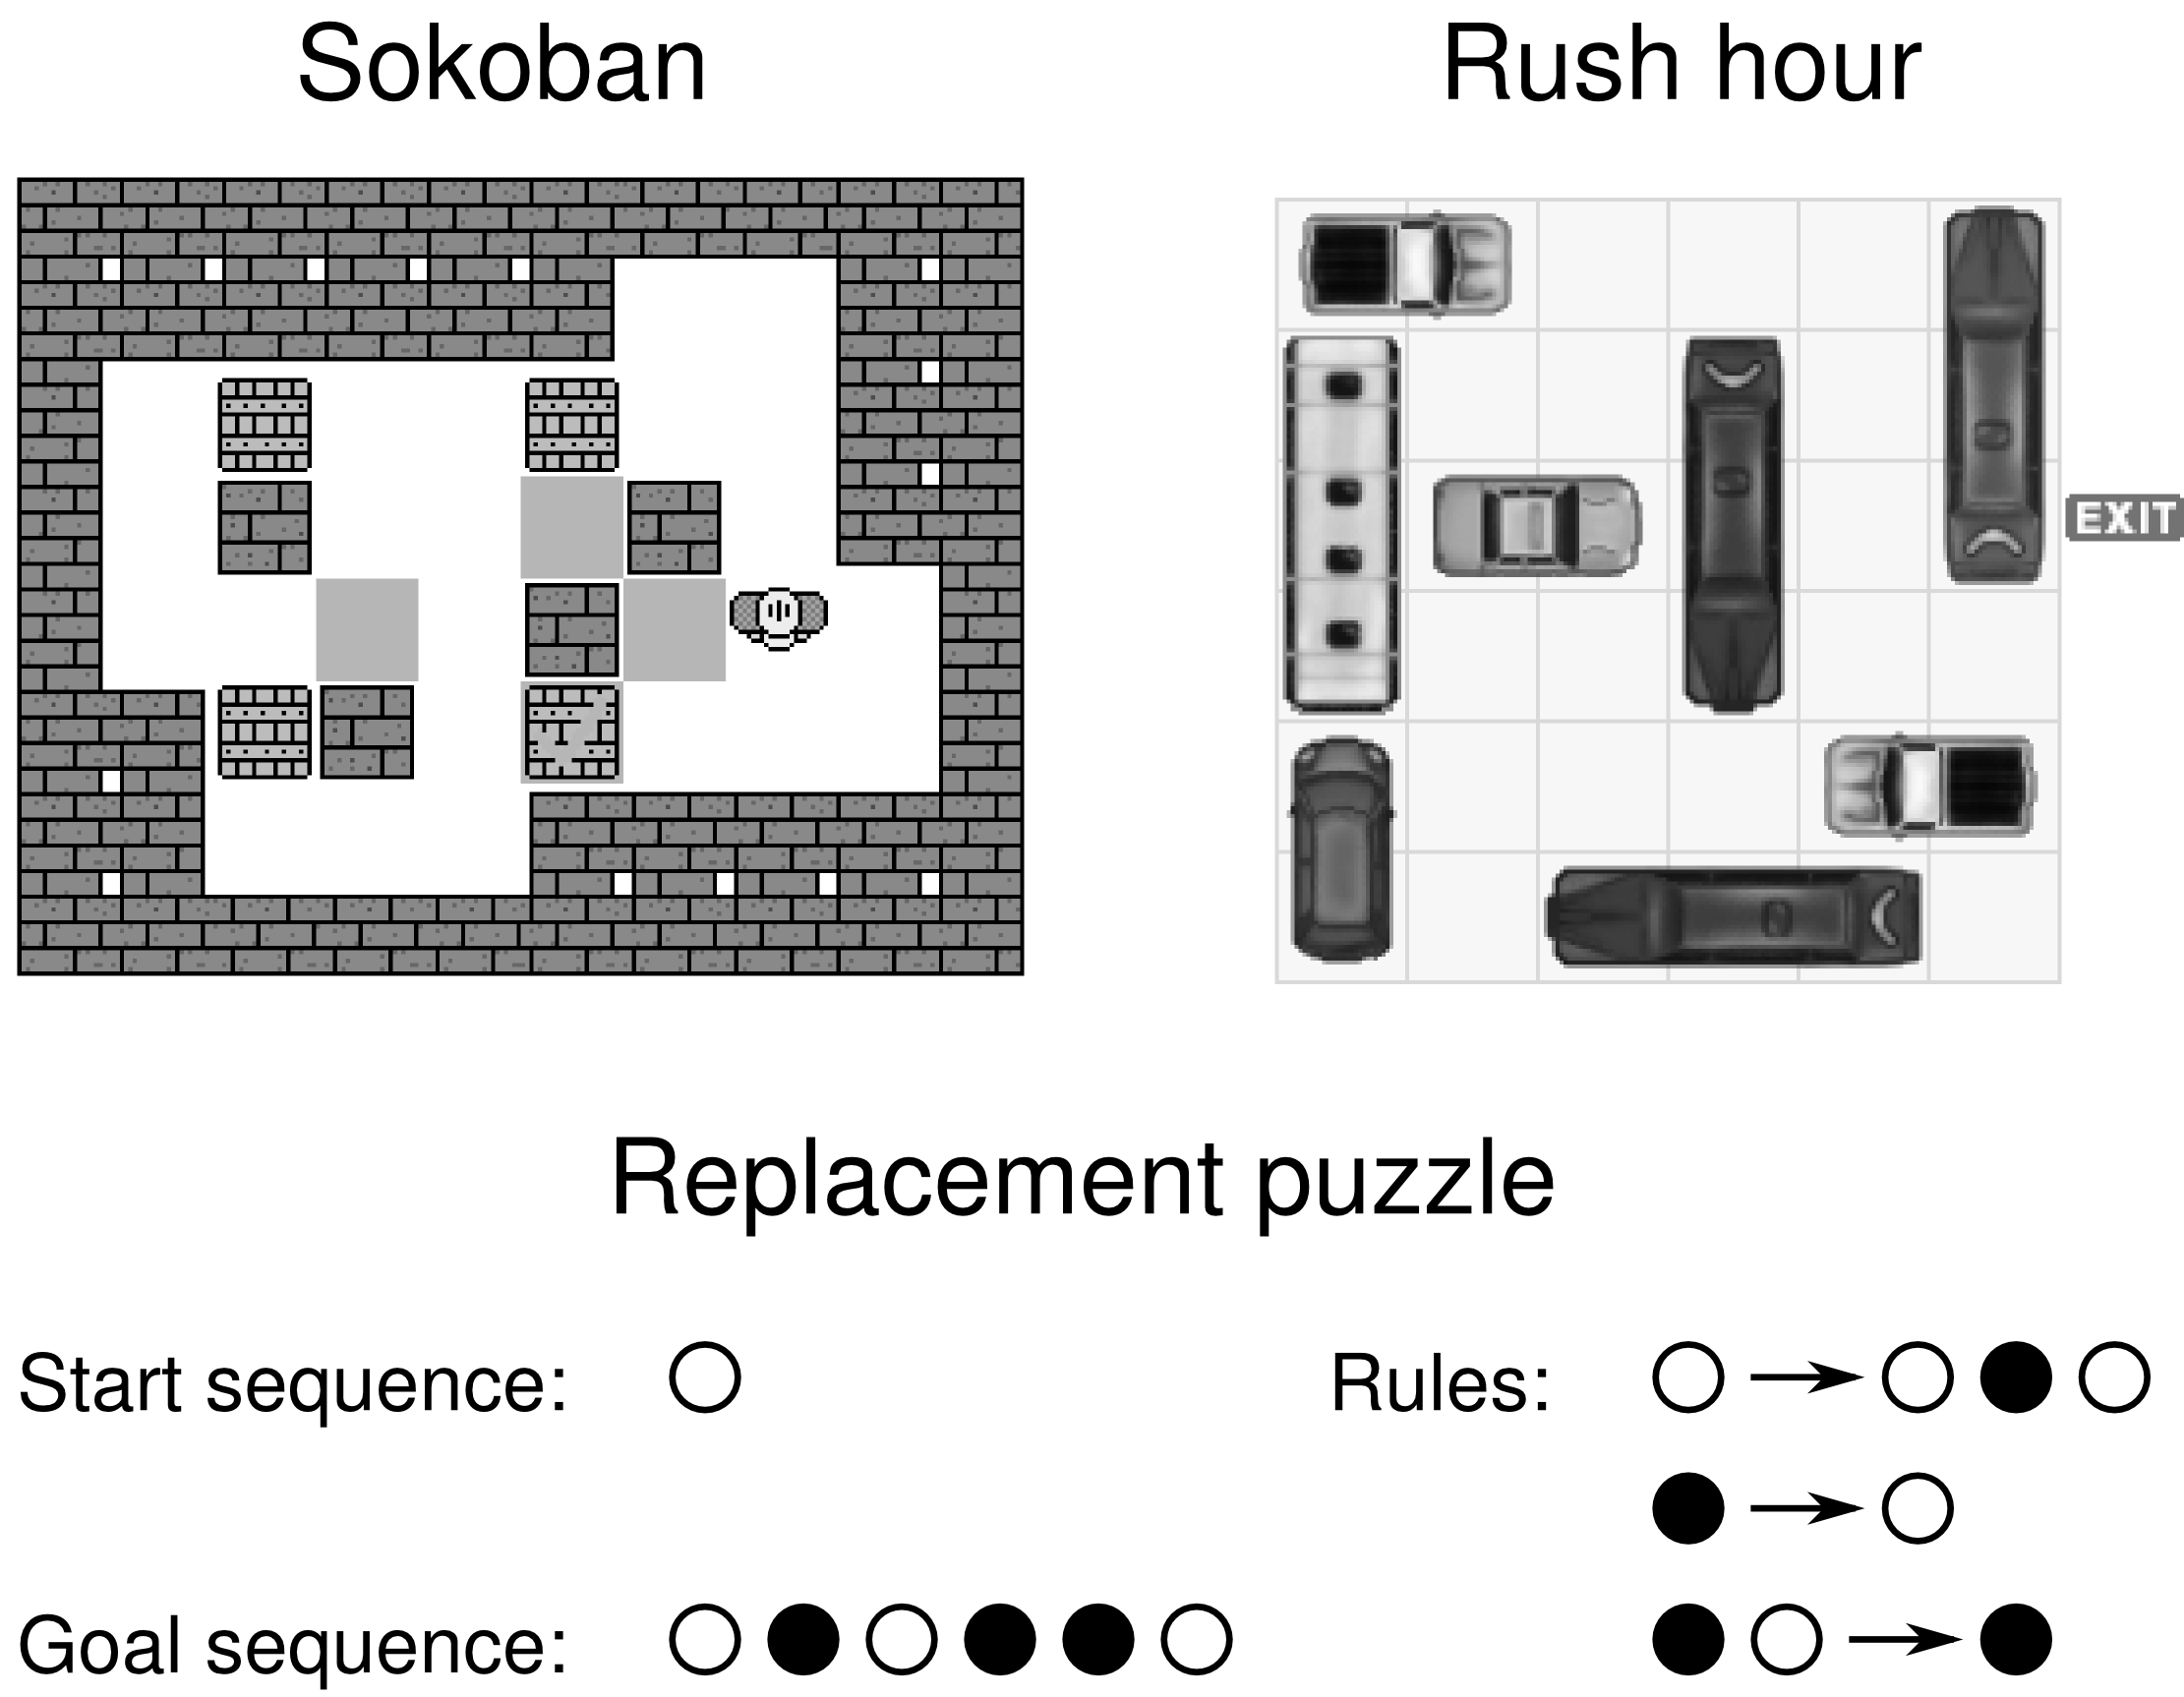
\includegraphics[width=\textwidth]{images/puzzles}
					\end{figure}
				\end{columns}
    		\end{frame}
    		\begin{frame}{Obtiažnosť ``posuvných'' hier}
    				\begin{block}{}
    					\begin{itemize}
    						\item data -- veľké rozdiely v obtiažnosti medzi inštanciami
    						\item tvrdia, že sú spôsobené štruktúrou stavového priestoru
    						\item vytvorili výpočtový model ľudského správania v stavovom priestore (kombinácia náhodného a optimálneho správania)
    						\item má iba jeden parameter -- jeho optimálna hodnota je takmer rovnaká pre všetky tri problémy
    					\end{itemize}
    				\end{block}
    				
    				$$score(s')=
\begin{cases}
d(s) & d(s') \geq d(s)\\
d(s) + B & d(s') < d(s)
\end{cases}$$
    		\end{frame}   
    		\begin{frame}{Obtiažnosť ``posuvných'' hier}
    			\begin{columns}
            		\column{0.5\linewidth}
\begin{table}[width=\textwidth]
\centering
\begin{tabular}{ll|l}
problem     & metric & $\rho$ \\ \hline
Rush hour   & SP     & 0.9        \\
            & $B = 25$ & 0.9        \\ \hline
Sokoban     & SP     & 0.41       \\
            & $B = 25$ & 0.61       \\ \hline
Replacement & SP     & 0.21       \\
puzzle      & $B = 25$ & 0.49      
\end{tabular}
\end{table}
				\column{0.5\linewidth}
    				\begin{block}{}
    					\begin{itemize}
    						\item model porovnávali aj s inými metrikami
    						\item výsledky sa líšia pre tri problémy
    						\item výsledky prinášajú nové otázky (napr. akú rolu hrá orientácia grafu stavov)
    					\end{itemize}
    		%We evaluated the model over collected data and compared it with other metrics for difficulty rating. The results differ for the three studied puzzles. In the case of the Rush hour puzzle, it is easy to predict difficulty even with the shortest path metric. For the Replacement puzzle, simple metrics do not work and the computational model does bring a significant improvement. The results open several new questions about problem solving, e.g., the role of directionality, or interaction between difficulty of local steps and global structure.
    				\end{block}
    			\end{columns}
    		\end{frame}     		  	
    		 		
      					
	\section{Gulička a strojové učenie}
		\subsection{Gulička}
			\begin{frame}{Pravidlá}
				\begin{block}{}
					\begin{itemize}
					    \item hracia plocha - 2D mriežka
					    \item medzi každými dvoma štvorčekmi môže byť stena
					    \item po okraji sú všade steny
					    \item $k$ modrých štvorčekov a jedna červená gulička
					    \item gulička sa hýbe v štyroch smeroch - hore, doprava, doľava a dole
					    \item pri pohybe sa gulička zastaví až keď narazí na stenu
					    \item gulička vezme modrý štvorček ak ním prejde, nemusí sa na ňom zastaviť
					    \item cieľ je pozbierať všetky modré štvorčeky
					\end{itemize}
				\end{block}
			\end{frame}
			\begin{frame}{}
				\begin{block}{}
					Tilt Maze (Gulička), podobné Quell-u
					
					Quell je v $\P$, dokázal Tejada\cite{tejada2014complexity}.
				\end{block}
			\end{frame}
			\begin{frame}{}
				\begin{figure}[h]
				    \centering
				    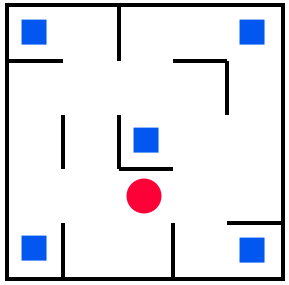
\includegraphics[width=0.6\textwidth]{images/gulicka}
				    %\caption{Sokoban instance}
				    %\label{fig:sokoban}
				\end{figure}
			\end{frame}
			\begin{frame}{Cieľ}
				\begin{block}{}
					\begin{itemize}
						\item zistiť ako ťažký je level pre človeka
						\item ako závísi jeho obtiažnosť od jeho atribútov
						\item resp. zistiť ktoré atribúty sú dôležité
					\end{itemize}
				\end{block}
			\end{frame}
		\subsection{Učenie s učiteľom}
			\begin{frame}{Učenie s učiteľom}
				\begin{block}{Dáta}
					Množina \emph{n} dvojíc \emph{x} - vstup, \emph{y} - očakávaný výstup.
				\end{block}
				\begin{block}{Cieľ}
					Predikovať výstup pre nové \emph{x}.
				\end{block}
				\begin{block}{Poznámka}
					Vo väčšine prípadov je $\vec{x}$ je vektor s \emph{m} hodnotami (atribútmi) a \emph{y} skalár.
				\end{block}
			\end{frame}
			\begin{frame}{Čo nás zaujíma}
				\begin{block}{}
					\begin{itemize}
						\item schopnosť modelu sa zovšeobecniť na nové dáta – \textbf{generalizácia}
						\item generalizácia sa dá merať chybou na nových dátach – \textbf{testovacia chyba}
						\item preto si delíme dáta na trénovaciu a testovaciu množinu
						\item testovacia chyba sa od trénovacej môže líšiť (niekedy málo, niekedy veľmi)			
					\end{itemize}				
				\end{block}
			\end{frame}			
		\subsection{Syntaktické vlastnosti}
			\begin{frame}{Atribúty}
				\begin{columns}						
					\column{0.7\linewidth}
						\begin{itemize}%[noitemsep]
						\item \texttt{checkpoint\_count}
						\item \texttt{tile\_count}
						\item \texttt{width}
						\item \texttt{reachable\_tile\_count}
						\item \texttt{reachable\_states\_count}
						\item \texttt{shortest\_path}
						\item \texttt{scc\_count}
						\item \texttt{scc\_checkpoint\_count}
						\item \texttt{reachable\_states\_log}
						\item ďalšie atribúty: \textcolor{bloodred}{počet slepých ciest, minimálny rez stavovým priestorom \ldots}
						\end{itemize}									
            		\column{0.3\linewidth}
						\begin{figure}[h]
							\centering
							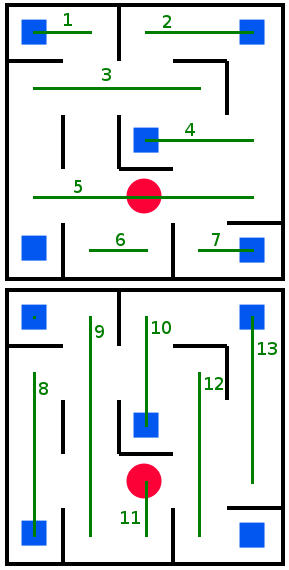
\includegraphics[width=0.9\textwidth]{images/gulicky2}
						\end{figure}
					\end{columns}
			\end{frame}
			\begin{frame}{\texttt{reachable\_states\_log}}
\begin{figure}[H]
    \centering
    \begin{tabular}[c]{cc}
        \begin{subfigure}[c]{0.45\textwidth}
            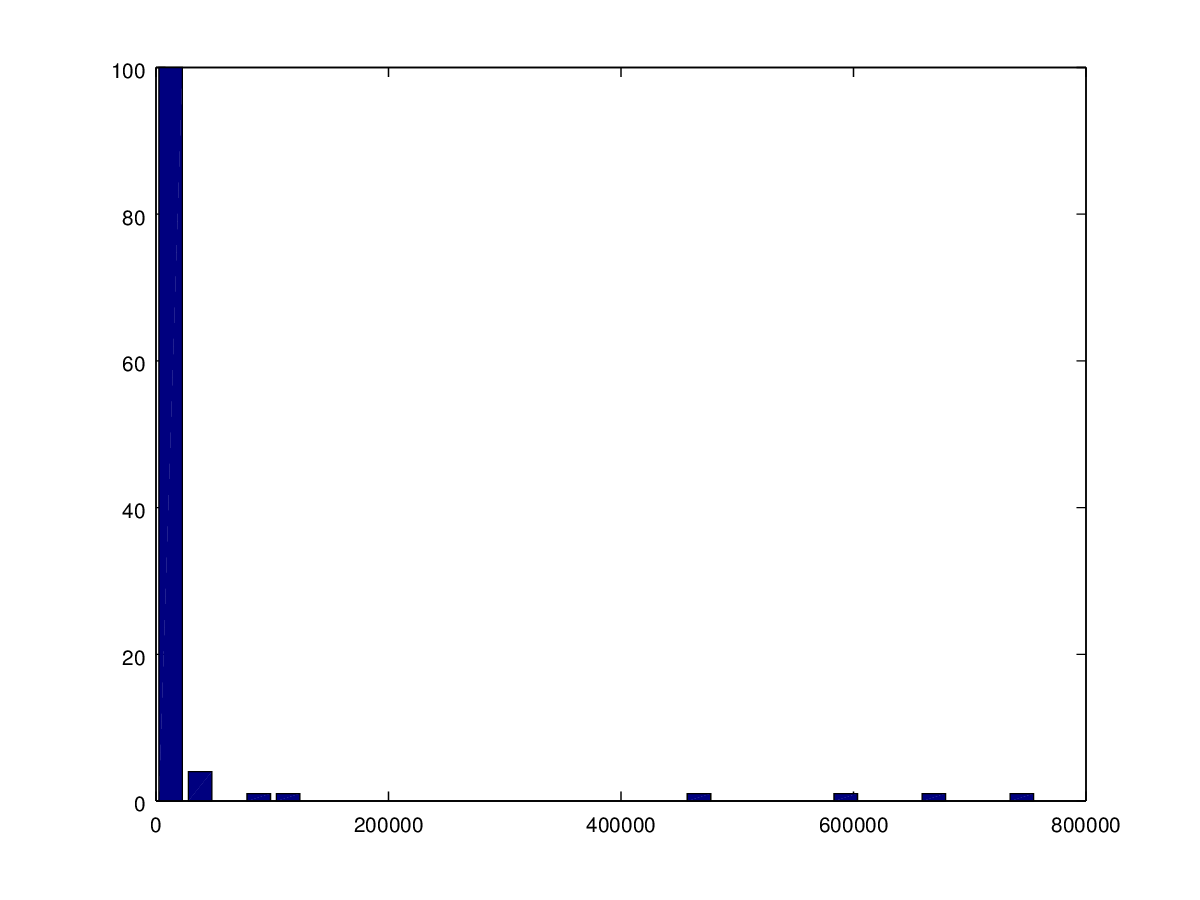
\includegraphics[width=\textwidth]{images/state.png}
            \caption{Počet dosiahnuteľných stavov}
            \label{fig:state}
        \end{subfigure}&
        \begin{subfigure}[c]{0.45\textwidth}
            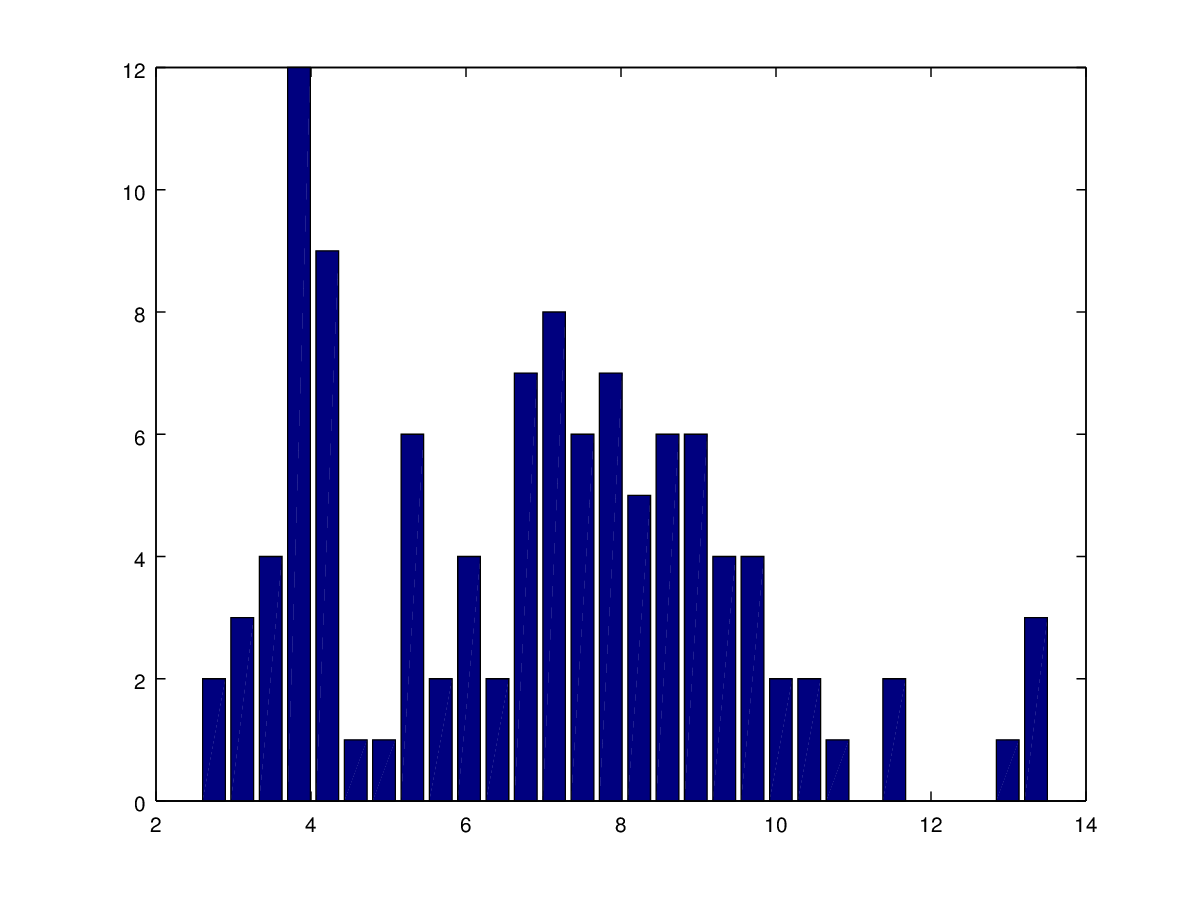
\includegraphics[width=\textwidth]{images/state_log.png}
            \caption{Logaritmus počtu dosiahnuteľných stavov}
            \label{fig:logstate}
        \end{subfigure}
    \end{tabular}
\end{figure}			
				
			\end{frame}
		\subsection{Časové dáta}
			\begin{frame}{Časové dáta}
\begin{table}[]
\centering
\tiny
\begin{tabular}{|c|c|c|c|c|c|c|c|c|c|c|c|c|}
\hline
\textbf{Login} & \textbf{221} & \textbf{223} & \textbf{225} & \textbf{227} & \textbf{228} & \textbf{229} & \textbf{230} & \textbf{231} & \textbf{232} & \textbf{233} & \textbf{234} & \textbf{235} \\ \hline
\textbf{U1}    & 11           & 12           &              &              & 64           &              &              &              &              &              &              &              \\ \hline
\textbf{U2}    & 2            & 28           & 45           & 59           & 41           &              &              & 27           & 100          &              & 107          &              \\ \hline
\textbf{U4}    & 25           &              &              & 205          & 12           & 29           &              & 32           & 116          & 55           & 89           &              \\ \hline
\textbf{U5}    &              & 5            & 9            &              & 45           & 160          &              & 53           & 41           &              &              &              \\ \hline
\textbf{U6}    & 10           & 11           &              &              &              &              &              &              &              &              &              &              \\ \hline
\textbf{U7}    & 5            & 11           & 10           & 41           & 16           & 49           & 204          & 28           & 39           & 89           & 85           & 283          \\ \hline
\textbf{U8}    & 5            & 11           &              & 43           & 54           &              &              &              &              &              &              &              \\ \hline
\textbf{U9}    & 8            & 11           & 18           & 45           & 20           & 82           &              & 53           &              &              &              &              \\ \hline
\textbf{U10}   & 44           & 15           &              &              & 26           &              &              &              &              &              &              &              \\ \hline
\textbf{U13}   & 9            & 12           & 19           & 37           & 49           & 28           & 128          & 42           & 66           & 50           & 37           & 273          \\ \hline
\textbf{U14}   &              & 65           & 33           & 86           & 65           & 135          &              &              &              &              &              &              \\ \hline
\textbf{U15}   &              & 18           & 38           &              & 32           & 96           &              &              &              &              &              &              \\ \hline
\textbf{U17}   & 4            &              &              &              &              &              &              &              &              &              &              &              \\ \hline
\textbf{U20}   & 22           & 28           & 35           & 48           & 31           & 141          & 270          & 124          & 163          & 41           & 176          & 179          \\ \hline
\textbf{U21}   & 35           & 42           & 129          &              & 63           &              &              & 37           &              &              &              &              \\ \hline
\textbf{U22}   & 11           & 29           & 32           &              & 31           &              &              & 51           &              &              &              &              \\ \hline
\textbf{U24}   & 10           & 20           & 19           &              & 194          &              &              &              &              &              &              &              \\ \hline
\textbf{U25}   & 26           & 16           & 23           & 96           & 23           & 57           & 514          & 15           & 99           & 120          & 268          &              \\ \hline
\textbf{U26}   & 23           &              &              & 86           & 22           & 58           & 306          & 37           & 80           & 51           & 144          & 184          \\ \hline
\end{tabular}
\end{table}				
			\end{frame}			
		\subsection{Experimentálne vyhodnotenie}
%			\begin{frame}{Možný výsledok}
%				\begin{block}{}
%					\* ak by sme napr. zistili, že časové dáta závisia iba od počtu políčok v levely, tak môžeme zhodnotiť, že hra Gulička je rovnako ťažká pre človeka ako pre počítač
%				\end{block}
%			\end{frame}		
			\begin{frame}{Výsledky}
				\begin{block}{}
					\begin{itemize}
						\item využili sme niekoľko bežných metód strojového učenia
						\item GridSearch -- natrénovanie metód
						\item skóre -- pre trénovaciu aj pre testovaciu množinu
						\item skóre -- \emph{Coefficient of determination}
						\begin{itemize}
							\item ak je $1.0$, tak parametre modelu sú najlepšie odhadnuté
							\item ak je $0.0$ model je rovnako dobrý ako random
							\item môže byť aj záporné, ak sa to naozaj zle natrénuje
						\end{itemize}
						$$R^2 = 1 - \frac{SS_{res}}{SS_{tot}} \qquad SS_{res} = \sum_i{e^2_i} \qquad SS_{tot}=\sum_i{y_i-\bar{y}}^2$$				
					\end{itemize}
				\end{block}
			\end{frame}	
			\begin{frame}{Výsledky}
					V tabuľke vidíme najlepšie parametre, trénovacie a testovacie skóre.
				\begin{table}[H]
					\centering
					\resizebox{\textwidth}{!}{%
					\begin{tabular}{|l|lcc|}
						\hline
						Method & Best params & Train score & test score \\
						\hline
						LinearRegression & -- & 0.60 & \textbf{0.54} \\
						Ridge & 'alpha': 100.0 & 0.55 & 0.48 \\
						Lasso & 'alpha': 0.10000000000000001 & 0.57 & 0.51 \\
						ElasticNet & 'alpha': 0.17782794100389229 & 0.57 & 0.50 \\ 
						SGDRegressor & 'alpha': 1.7782794100389228 &0.52 & 0.44\\
						SVR & 'kernel': 'rbf', 'gamma': 0.001, 'C': 1.0 & 0.35 &0.29 \\
						RandomForestRegressor & 'n\_estimators': 15 & \textbf{0.76} & 0.48\\
						KNeighborsRegressor & 'n\_neighbors': 15, 'algorithm': 'auto' & 0.53 & 0.49\\
\hline
					\end{tabular}}
				\end{table}
			\end{frame}
			\begin{frame}{Metóda ostraňovania parametrov}
				\begin{block}{}
					\begin{itemize}
						\item každý jeden atribút sme skúsili odstrániť
						\item potom sme každú metódu natrénovali znova
						\item v nasledujúcich tabuľkách uvidíme trénovacie a testovacie skóre jednotlivých metód
					\end{itemize}
				\end{block}
			\end{frame}
			\begin{frame}{Metóda ostraňovania parametrov -- trénovacie skóre}
				\begin{table}[H]
					\centering
					\resizebox{\textwidth}{!}{%
					\begin{tabular}{|l|llllllll|}
						\hline
						Feature                  & LR & Ridge & Lasso & EN & SGDR & SVR  & RFR & KNR \\
						\hline
						checkpoint\_count        & 0.60             & 0.56  & 0.57  & 0.57       & 0.53         & 0.52 & 0.74                  & 0.53                \\
						tile\_count              & 0.59             & 0.56  & 0.57  & 0.57       & 0.53         & 0.52 & 0.78                  & 0.53                \\
						width                    & 0.58             & 0.55  & 0.57  & 0.55       & 0.52         & 0.50 & 0.77                  & 0.55                \\
						reachable\_tile\_count   & 0.50             & 0.45  & 0.49  & 0.44       & 0.42         & 0.44 & 0.74                  & 0.52                \\
						scc\_count               & 0.47             & 0.36  & 0.00  & 0.00       & 0.35         & 0.39 & 0.77                  & 0.47                \\
						scc\_checkpoint\_count   & 0.37             & 0.14  & 0.00  & 0.00       & 0.10         & 0.36 & 0.71                  & 0.47                \\
						shortest\_path           & 0.37             & 0.15  & 0.00  & 0.00       & 0.11         & 0.17 & 0.64                  & 0.42                \\
						reachable\_states\_count & 0.36             & 0.23  & 0.00  & 0.00       & 0.18         & 0.19 & 0.47                  & 0.42                \\
						\textbf{reachable\_states\_log}   & \textbf{0.00}             & \textbf{0.00}  & \textbf{0.00}  & \textbf{0.00}       & \textbf{0.00}         & \textbf{0.00} & \textbf{0.00}                  & \textbf{-0.13}				\\
						\hline            
					\end{tabular}}
				\end{table}			
			\end{frame}
			\begin{frame}{Metóda ostraňovania parametrov -- testovacie skóre}
				\begin{table}[H]
					\centering
					\resizebox{\textwidth}{!}{%
					\begin{tabular}{|l|llllllll|}
						\hline
						Feature                  & LR & Ridge & Lasso & EN & SGDR & SVR   & RFR & KNR \\
						\hline
						checkpoint\_count        & 0.57             & 0.45  & 0.51  & 0.50       & 0.42         & 0.43  & 0.51                  & 0.47                \\
						tile\_count              & 0.53             & 0.46  & 0.51  & 0.50       & 0.43         & 0.44  & 0.52                  & 0.48                \\
						width                    & 0.53             & 0.47  & 0.52  & 0.50       & 0.44         & 0.43  & 0.46                  & 0.47                \\
						reachable\_tile\_count   & 0.45             & 0.41  & 0.47  & 0.43       & 0.37         & 0.41  & 0.40                  & 0.34                \\
						scc\_count               & 0.44             & 0.34  & -0.04 & -0.04      & 0.32         & 0.39  & 0.31                  & 0.36                \\
						scc\_checkpoint\_count   & 0.51             & 0.12  & -0.04 & -0.04      & 0.07         & 0.31  & 0.37                  & 0.40                \\
						shortest\_path           & 0.50             & 0.13  & -0.04 & -0.04      & 0.08         & 0.22  & 0.38                  & 0.39                \\
						reachable\_states\_count & 0.49             & 0.24  & -0.04 & -0.04      & 0.18         & 0.23  & 0.09                  & 0.40                \\
						\textbf{reachable\_states\_log}   & \textbf{-0.04}            & \textbf{-0.04} & \textbf{-0.04} & \textbf{-0.04}      & \textbf{-0.04}        & \textbf{-0.02} & \textbf{-0.06}                 & \textbf{-0.31}  		\\
						\hline            
					\end{tabular}}
				\end{table}			
			\end{frame}
			\begin{frame}{Záver}
				\begin{block}{}
					\begin{itemize}
						\item môžeme predpokladať, že obtiažnosť levelu aspoň mierne závisí od daných syntaktických vlastností
						\item zároveň logaritmus počtu dosiahnuteľných stavov ovplyvňuje obtiažnosť najviac (z daných parametrov)
						\item do budúcnosti -- získať viac dát, nájsť dáta pre problémy, ktoré majú rovnaké alebo podobné parametre				
					\end{itemize}
				\end{block}
			\end{frame}					
										          
            
	\section{Koniec}
		\subsection{Do budúcnosti}
			\begin{frame}{Čo ďalej?}
				\begin{block}{}
					\begin{itemize}
						\item využiť iné metódy (neurónové siete \ldots)
						\item skúsiť iné prístupy (štatistické testy \ldots)
						\item využiť dáta o jednotlivých užívateľoch (\emph{collaborative filtering})
						\item hľadať ďalšie vlastnosti (minimálny rez \ldots)
						\item vyskúšať iné Puzzle (Rush Hour \ldots)
					\end{itemize}
				\end{block}
			\end{frame}
		\subsection{Zdroje}                
            \begin{frame}[allowframebreaks]{Zdroje}
			\footnotesize
				\nocite{*}
				\bibliographystyle{apalike}
				\bibliography{literatura.bib} 
            \end{frame}
	
        \subsection{Podakovanie}                
            \begin{frame}
				\vfill
				\begin{center}
					\huge\bfseries
					Ďakujem za pozornosť
					\vfill
				\end{center}
			\vfill
            \end{frame}
	\section{}
		\subsection{Metódy}
			\begin{frame}{}
				\begin{itemize}%[noitemsep]
				\item LinearRegression -- obyčajná lineárna regresia, nemá parametre
				\item Ridge  -- linear least squares a L2 regularizácia -- tá je kontrolovaná parametrom \texttt{alpha} ktorý GridSearch skúša od $10^{-3}$ po $10^3$.
				\item Lasso -- L1 regularizácia -- kontrolovaná \texttt{alpha} podobne ako pri Ridge
				\item ElasticNet -- L1 + L2 regularizácia -- tiež kontrolovaná \texttt{alpha}
				\item SGDRegressor -- stochastický gradient descent -- tiež skúšam meniť \texttt{alphu}
				\item SVR -- je vlaste SVMko pre regresiu, skúšam dva rôzne kernely \texttt{linear} a \texttt{rbf}, pre oba skúšam rôzne \texttt{C}čka a pre \texttt{rbf} aj \texttt{gammy}.
				\item RandomForestRegressor -- les stromov pre regresiu, hlavným parametrom je počet stromov v lese
				\item KNeighborsRegressor -- určuje na základe niekoľkých najbližších susedov, počet susedov si určím GridSearchom
\end{itemize}
			\end{frame}            
\end{document}